%%%%%%%%%%%%%%%%%%%%%%%%%%%%%%%%%%%%%%%%%%%%%%%%%%%%%%%%%%%%%%%%%%%%%%%%%%%%%%%%
%2345678901234567890123456789012345678901234567890123456789012345678901234567890
%        1         2         3         4         5         6         7         8

\documentclass[letterpaper, 10 pt, conference]{ieeeconf}  % Comment this line out
                                                          % if you need a4paper
%\documentclass[a4paper, 10pt, conference]{ieeeconf}      % Use this line for a4
                                                          % paper

\IEEEoverridecommandlockouts                              % This command is only
                                                          % needed if you want to
                                                          % use the \thanks command
\overrideIEEEmargins
\usepackage{graphicx}
\usepackage{sidecap}
% See the \addtolength command later in the file to balance the column lengths
% on the last page of the document



% The following packages can be found on http:\\www.ctan.org
%\usepackage{graphics} % for pdf, bitmapped graphics files
%\usepackage{epsfig} % for postscript graphics files
%\usepackage{mathptmx} % assumes new font selection scheme installed
%\usepackage{times} % assumes new font selection scheme installed
%\usepackage{amsmath} % assumes amsmath package installed
%\usepackage{amssymb}  % assumes amsmath package installed

\title{\LARGE \bf
Byzantine Chain Replication
}

%\author{ \parbox{3 in}{\centering Huibert Kwakernaak*
%         \thanks{*Use the $\backslash$thanks command to put information here}\\
%         Faculty of Electrical Engineering, Mathematics and Computer Science\\
%         University of Twente\\
%         7500 AE Enschede, The Netherlands\\
%         {\tt\small h.kwakernaak@autsubmit.com}}
%         \hspace*{ 0.5 in}
%         \parbox{3 in}{ \centering Pradeep Misra**
%         \thanks{**The footnote marks may be inserted manually}\\
%        Department of Electrical Engineering \\
%         Wright State University\\
%         Dayton, OH 45435, USA\\
%         {\tt\small pmisra@cs.wright.edu}}
%}

\author{Amith Gopal and Manish Shambu% <-this % stops a space
}


\begin{document}



\maketitle
\thispagestyle{empty}
\pagestyle{empty}


%%%%%%%%%%%%%%%%%%%%%%%%%%%%%%%%%%%%%%%%%%%%%%%%%%%%%%%%%%%%%%%%%%%%%%%%%%%%%%%%
\begin{abstract}

Byzantine failures are defined as arbitrary, unpredictable failures of a process from its assumed behavior based on the algorithm it is supposed to execute. To address and mitigate the Byzantine failures, designing chain replication protocols is the way to go which detects and addresses the Byzantine failures. Chain Replication is a special primary backup system in which the servers are linearly ordered to form a chain with the primary at the end. Byzantine fault tolerant (BFT) state machine replication is a promising technique for using redundancy to improve integrity and availability and that it is practical in that it adds modest latency and can proactively recover from faults.

\end{abstract}


%%%%%%%%%%%%%%%%%%%%%%%%%%%%%%%%%%%%%%%%%%%%%%%%%%%%%%%%%%%%%%%%%%%%%%%%%%%%%%%%
\section{INTRODUCTION}

Byzantine fault tolerance was invented in the late 70s, when NASA initiated a project to build computers that are reliable enough to fly aircraft. Today Byzantine fault tolerance continues to be used in flying aircraft and space shuttles, but it also finds new application in distributed applications. We believe that Traditional Byzantine fault tolerant algorithms will be increasingly important in the future because malicious attacks and software errors are increasingly common and can cause faulty nodes to exhibit arbitrary behavior.
Traditional Byzantine fault tolerant Machines require 3t + 1 replicas. This is too costly for an organization to implement such protocols. Encryption pushes up the computing or CPU costs. Some protocols make complex assumptions which makes it very hard to implement and debug. Existing chain replication protocols require accurate failure detection.
In order to detect and tolerate the Byzantine failures and overcome the problems that the traditional chain replication protocols pose, we intend to develop an easily reconfigurable Chain Replication protocol called Shuttle which requires only 2t + 1 replicas and does not require accurate failure detection.
Asynchronous Distributed Systems are more suitable for real world scenarios since it does not make any assumptions about time and order of event sin distributed systems. Considering deploying a scalable and most robust fault tolerant system, we present protocols for an Asynchronous Systems.
Today’s block chain technology requires Byzantine fault tolerant protocols to be more Robust and Durable. The main goals of our Byzantine fault tolerant system would be Integrity, Confidentiality and Availability.

%%%%%%%%%%%%%%%%%%%%%%%%%%%%%%%%%%%%%%%%%%%%%%%%%%%%%%%%%%%%%%%%%%%%%%%%%%%%%%%%
\section{RELATED WORK}

State machine replication involves costly operations in maintaining state. Making the machines independent or stateless gives a lot of robustness to a system, when it encounters failures and recovers back.
BChain-3 and BChain-5 protocols require 3t +1 and 5t+1 replicas. Respectively to tolerate t fault tolerant machines. BChain uses chain replication while faulty replicas are diagnosed and eventually reconfigured. ByzID used intrusion detection methods to build a Byzantine failure detector. Faulty replicas are detected immediately, and performance attack can be perfectly handled. Byzantine chain replication employs a centralized trusted computing base to tolerate Byzantine failures.

\subsection{Fault Tolerant approaches}
The rollback recovery approaches such as message logging and check- pointing assume the existence of stable storage and optionally employ a notary service, but do not have surrogates. Application processes save state and/or messages in stable storage while running. When an application process crashes, a new one loads the state and messages from stable storage and recover the system to a consistent state. Since there are no surrogates, these approaches can take considerable time to recover from failures.

The primary-backup approach models each application process as a primary and implements stable storage that stores the state of the primary using t backups. The t backups also serve as surrogates, which can take over from the primary when it fails. Unlike rollback recovery approaches, the primary-backup approach recovers quickly from failures, because the surrogates are kept up-to-date with the primary.

The state machine replication approach replicates the state but not the result as in primary backup. Each replica executes a command to reach a particular state. There are two variants of state machine replication, Leader based and symmetric.

The transaction processing approach is designed to maintain a consistent state when executing transactions in distributed databases. Each participant in a transaction can execute multiple operations, and the operations may differ among the participants. When we treat the execution of each input as a transaction, transaction processing can be used to implement fault tolerant distributed applications. More specifically, we can replicate each application process, and designate one replica to serve as the coordinator. Input messages are submitted to the coordinator, which coordinates the replicas to handle each input message as a transaction.

\subsection{Translation Techniques}
The idea of automatically translating crash-tolerant systems into BFT systems can be traced back to the mid-eighties. Gabriel Bracha presents a translation mechanism that transforms a protocol tolerant of up to t crash failures into one that tolerates t Byzantine failures. Brian Coan also presents a translation that is similar to Bracha’s.

Toueg, Neiger and Bazzi worked on an extension of Bracha’s and Coan’s approaches for translation of synchronous systems . Mpoeleng et al. present a scalable translation that is also intended for synchronous systems, and transforms Byzantine faults to so-called signal-on-failure faults.

\subsection{Cost Reduction Approaches}
One of the first systems to consider asynchronous Byzantine replication for practical deployment is PBFT, which demonstrates the practicality of a BFT version.

A notable series of optimization follows the principle of separation of concerns. It separates agreement from execution and observes that it is not necessary to have 3t + 1 full replicas. The authors suggest a model with 2t + 1 execution nodes  and 3t + 1 agreement nodes. ZZ further optimizes by noticing that replicas can be turned off and treated as “slow” in normal runs. To tolerate t Byzantine failures, a ZZ system employs t + 1 execution nodes and 3t + 1 agreement nodes in normal runs. It brings up the other replicas from an hibernated state when required.

Our affordable replication approach, called Shuttle, reduces the replication cost by relying on an external configuration service for liveness when failures occur. The Shuttle protocol uses only t + 1 replicas and t witnesses to make progress when failures do not occur while preserving safety against up to t Byzantine failures. However, when it is possible to make a stronger assumption about the adversary, we can eliminate witnesses and use t+1 replicas alone to preserve safety. With the stronger assumption, we can use a cheaper cryptographic primitive and reduce the computational cost of the protocol. Shuttle never rolls back any transaction.


%%%%%%%%%%%%%%%%%%%%%%%%%%%%%%%%%%%%%%%%%%%%%%%%%%%%%%%%%%%%%%%%%%%%%%%%%%%%%%%%

\section{Design Description}
Our basic idea is to establish safety and liveness properties in a distributed system. There exists a configuration service engine which creates a replicated chain initially. This initial replicated chain will be in the active state wherein all the replicas/objects are running. Once there is a faulty replica, the chain becomes immutable and now the configuration service switches to a different configuration which has an ordered set of replicas within it. This continues to happen, until there is a configuration which has all the correct replicas which satisfies the liveness property.

The logical components we categorize the system in order to explain the design is as following:\smallskip

OLYMPUS: A centralized server which manages the configuration of many replicated servers in the group. It maintains a map of all the configurations with the replicated servers in that configuration. Also, it handles failure events generated by some replicas and triggers a configuration change.\smallskip

GROUPS: A replicated set of servers is collectively called a Group. \smallskip

CHAIN: This is an arrangement of the replica groups. It is also called as Group Chain. Inside a group chain, it is logically divided into a replica chain followed by a witness chain. Each chain begins with a head and ends with a tail.
The communication using a chain pattern is preferred since the communication here reduces the bandwidth consumption to approximately half compared to broadcasting.\smallskip

LEADER: The head replica of the chain is the Leader.\smallskip

After the logical components, it is very important to state the different types of protocols existing in the system:\smallskip

FAILURE DETECTION PROTOCOL: Every member runs this protocol in the active state, monitors messages and raises a detection or a suspicion event on the occurrence of an unexpected event.\smallskip

ACKNOWLEDGEMENT RETRANSMISSION PROTOCOL: This protocol is used to maintain liveness in the system and prevent omission. This is basically involves resending the messages until the Group sending the message receives an acknowledgment or the message being sent is in the history of the receiver group. \smallskip

STATE TRANSFER PROTOCOL: This protocol is used to preserve Safety in the system by transferring history/state of one configuration to the new configuration. \smallskip

ORDER PROTOCOL : This protocol states that no correct replicas will store the same message in a different order in their history.\smallskip

REQUEST PROCESSING PROTOCOL: The leader takes in requests, verifies it and sends the message to all the replicas and expects the signed output from each of these replicas. The order proof created for each request is appended to the history in each of the replicas. Order proof is basically a signed statement by a replicas which contains the message along with the identifier.\smallskip

RECONFIGURATION PROTOCOL: It is sent by a replica to the Olympus on facing a timeout/crash failure asking for the Olympus to create a new configuration.\smallskip

WEDGE REQUEST: On receiving the reconfiguration request, the olympus fires a wedge request to all the replicas.\smallskip

WEDGE RESPONSE: On receiving the Wedge request, the replicas become immutable and send their history to the Olympus in a Wedge Response.\smallskip

CATCH-UP PROTOCOL: It is executed by the Olympus after the wedge response is got by all the replicas in the configuration. After finding the longest history from the wedge response, the olympus sends this longest history to all the replicas in the configuration to catch up with this longest history. \smallskip

CONFIGURATION MANAGEMENT PROTOCOL: It is run by the Olympus where a new configuration is created and uses the State transfer protocol to seamlessly transfer the history from one configuration to the other.\smallskip

Since our system is representation of state machine replication, the following are the states that a configuration goes through.

Also described about each state is the state transition. \smallskip

NEW STATE: This is the state every configuration begins with. State transfer protocol is used in this state to change to the next state.\smallskip

ACTIVE STATE: After the transferring of the state, the new configuration becomes ready and makes a transition to the Active state. The active state is the busiest state wherein the Acknowledgement retransmission protocol, Request processing protocol, failure detection protocol runs.\smallskip

PASSIVE STATE: Once the Failure Detection Protocol detects a failure, the configuration enters the Passive State. In this state, change of configuration protocol is fired to determine a new configuration to ensure liveness. \smallskip

\begin{figure*}
  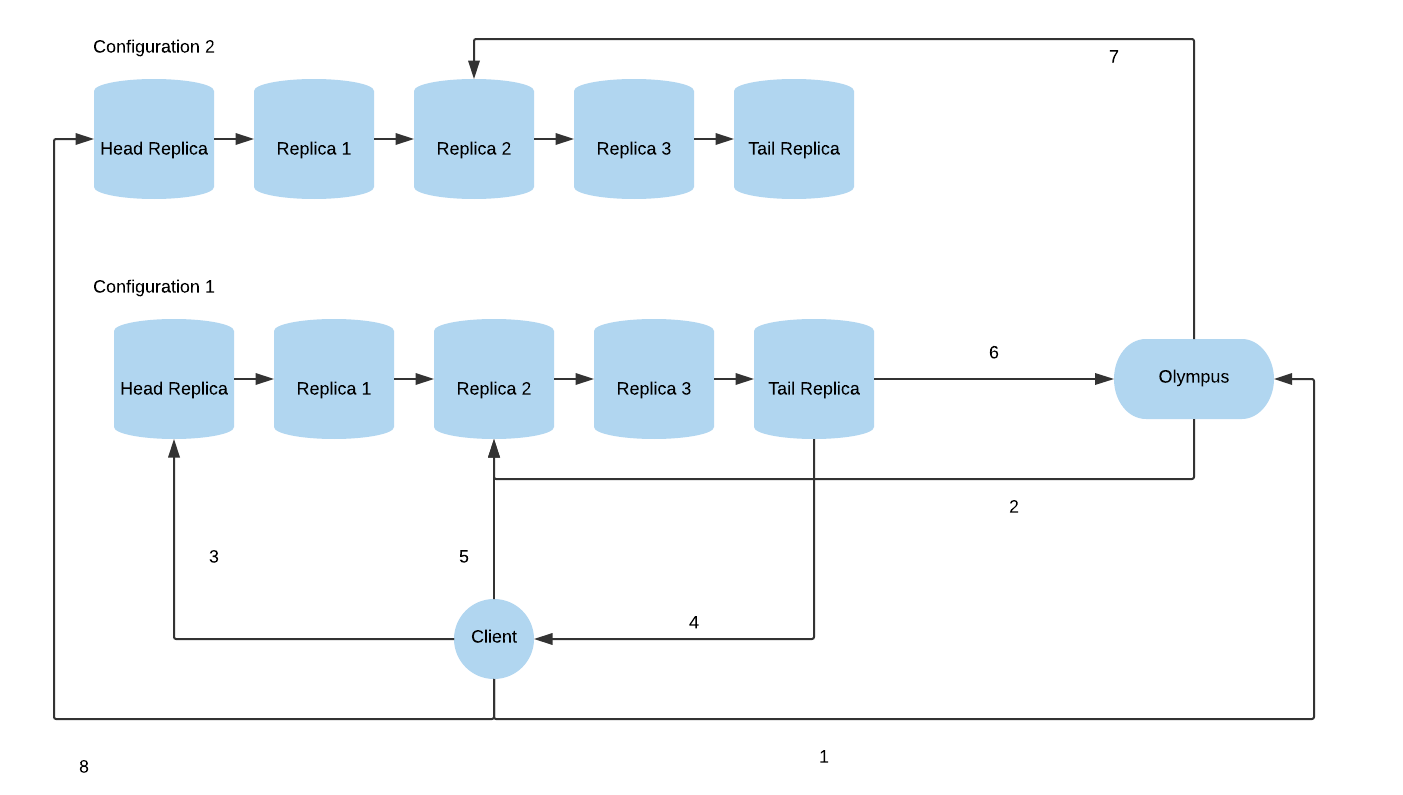
\includegraphics[width=\linewidth]{Architecture}
  \centering
  \caption{Architecture and messages}
  \label{}
\end{figure*}

Figure 1 shows the design architecture and messages exchanged between the client, replicas and the Olympus node. The message interactions are numbered.
1. The client contacts the Olympus initially to install a new configuration.
2. Olympus installs a new configuration on the replicas.
3. Once the configuration is installed, the client queries the replica chain.
4. The tail replica replies back to the client with a result.
5. If the tail does not reply to the client within a given time, the client sends request to all the replicas.
6. If a suspicion is triggered, the FDS makes the chain contact the Olympus to install a new configuration.
7. Olympus creates and installs a new configuration.
8. The client queries the new configuration.
\smallskip

\textit{Failure free behavior}

Assuming every replica is good, a client requests a transaction to be performed by sending the request to the head of the replica. The head of the replica verifies the request, processes it and creates an order statement. An order statement is of the form (REQUEST NUMBER, REQUEST, REPLICA ID).
It also creates a result statement of the form (REQUEST NUMBER, RESULT, HASH(RESULT), REPLICA ID). The above two statements are combined together to form a forward Shuttle. This forward shuttle is sent to the next replica. 

The next replica follows the same operations as the head replica. It creates a forward shuttle, appends to the forward shuttle sent by the head and sends it to its next replica. This continues to the next replica until it reaches the tail. The tail executes the operations and sends the list of the result proofs along with the result to the client. The client obtains the result.

After sending to the client, the tail stores the result proof, order proof, action and the result in it's history and creates a Result Shuttle. A result shuttle comprises of (List(Order statements), List(Result Statements), result, action). The result shuttle now is sent back towards the head through the chain. Along the chain, each replica stores the information from the result shuttle in it's history just like the tail did.

\textit{Behavior during a crash failure}

Assuming there's a crash in one of the replicas or there is a timeout, the replica will not be able to send the forward shuttle or the result shuttle. This causes the replica waiting for the result shuttle to timeout and send an reconfiguration request to the Olympus. The Olympus on receiving of the reconfiguration request sends a wedge request to all the replicas in the current configuration. The replicas on receiving of the wedge request will change the state of the replica to an immutable state from the active state. The replica send a wedge response to the Olympus along-with their history. Olympus on receiving these responses will figure out the longest history amongst all the replicas. Olympus sends a catch up request to all the replicas with this longest history. The replicas which are lagging behind catch up by executing all the operations present in the history which they have not yet performed. This catch-up request is used to use the same replicas in the previous configuration as part of the new configuration.

Once this is done, the olympus creates a new configuration with the same number of replicas. The longest history that is obtained is sent to all the replicas in the new configuration. All the replicas now will have the same state as it was before.

\textit{Timeout/ Crash failures}

Client starts a timer after requesting an operation to be done to the head. If the timer expires, the client then broadcasts the operation to all the replicas in the configuration. Each of those replicas on receiving the operation will:

a. Check if the operation is in the history
   If present in the history, then it replies to the client with result proofs corresponding to the action.
b. If not present in the history, then it forwards the request to the head and starts a timer.
    If the operation is present in the head's history then it simply responds to the replica with a result proof and a result. Otherwise, it starts a new request by creating a forward shuttle and sending it along the chain.
    
On timeout in both the cases mentioned above, the reconfiguration protocol is fired from one of the replicas. The olympus then creates a new configuration as mentioned previously.

Once the new configuration is created by the olympus, it responds to the client (which has been polling it continuously for a new configuration) with a new configuration. Client now sends the request to the head of this new configuration.

\textit{Behavior during Byzantine faults}

Assuming one of the replicas to be byzantine, it can behave in the following ways:

1. Computes some other operation apart from the one that is specified.
2. Creates an order statement in which one order corresponds to two different operations. This must not happen since it goes against the basic principle of our protocol which states that there must be a unique order for an operation.

For the first scenario, even though some replicas are byzantine, let's say 't', when the tail sends the result proofs and the result to the client with some wrong results, the client ignores the wrong results as long it obtains a majority of right results. In this way, Shuttle is byzantine fault tolerant.

For the second scenario, while the forward shuttle is passing through the chain, the replica detects the assignment of 2 different operations to a single order number. This triggers a reconfiguration protocol to the Olympus where a new configuration is created which makes sure the progress of further operations is continued.

%%%%%%%%%%%%%%%%%%%%%%%%%%%%%%%%%%%%%%%%%%%%%%%%%%%%%%%%%%%%%%%%%%%%%%%%%%%%%%%%
\section{How 2t + 1?}
This section describes a detailed explanation of why the shuttle protocol require only 2t + 1 replicas to support t faults.\smallskip

The architecture of the shuttle protocol separates agreement that orders request from execution unlike the earlier BFT protocols such as Bchain3. Separating agreement from execution also allows a general privacy firewall architecture to protect confidentiality through replication. Replication in previous systems hurts confidentiality because exploiting the weakest
replica can be sufficient to compromise the system. A simple majority of correct servers suffices to mask Byzantine faults among execution servers. 2t+1 replicas can tolerate t faults. (t+1 servers form a majority group.) A privacy firewall between the agreement nodes and the execution nodes filters the  minority answers from replies rather than sending these incorrect replies to clients.\smallskip

For a general Byzantine Fault tolerant system, assuming 't' failures occur, to maintain uninterrupted running of the system 3t+1 replicas are preferred. The reason for this is 't' more correct replicas are assumed to be lagging behind others(this assumption is done for failure masking). Also, t+1 more replicas are required for the authenticity of the request. Now if we can neglect the failure masking since it is not preferred for most of the practical applications as it adds requirement for more replicas, our system will now have only 2t+1 replicas. The new architecture also has a centralized server called Olympus to issue commands in order. Witnesses do not hold application state nor perform application operations.

The replication of data that happened in the earlier protocols were dependent on the other. So, if one replica became faulty, it corrupted the other replicas by issuing wrong data and that wrong data is further replicated (what happens in the case of Byzantine Generals problem). But in chain replication, the data gets replicated independently.

%%%%%%%%%%%%%%%%%%%%%%%%%%%%%%%%%%%%%%%%%%%%%%%%%%%%%%%%%%%%%%%%%%%%%%%%%%%%%%%%
\section{Implementation}

A high level language called DistAlgo was chosen. The reasons for choosing this are:
1. Creation of multiple processes required simple implementation.
2. Ease in sending and receiving messages.
3. Handling of multiple processes simple.
4. Timers are simple to understand and easy to implement.
5. Language based on Python which made it easy to understand and implement.

We created multiple processes using Distalgo to imitate multiple replicas.
The design mentioned in the above section is a generic design of any chain replication protocol. Some disadvantages of most of the chain replication protocols is the amount of overhead which is caused on the Configuration service when there is a configuration change request.
We will try to solve this using Shuttle protocol. The basic idea of a shuttle protocol is to increase the efficiency and the latency by having minimum number of replicas and make the reconfiguration process fast.

Our implementation includes the following modules:

OLYMPUS: It is a class implemented in DistAlgo. Only one instance of Olympus is spawned. It creates new configurations. It stores information about the current configuration which includes information about the replicas. 

REPLICA MODULE: It is a skeleton for instantiating a process for a replica. It contains data structures which is used to store the incoming messages and outgoing messages. They also encapsulate many variables which indicate the state of the system, number of processes verified and executed, the addresses of the client and olympus servers, private and public keys etc.

CLIENT MODULE: 

This class is implemented in DistAlgo which can be used to spawn many clients. It stores the address of the Olympus and information about the current configuration.  


%%%%%%%%%%%%%%%%%%%%%%%%%%%%%%%%%%%%%%%%%%%%%%%%%%%%%%%%%%%%%%%%%%%%%%%%%%%%%%%%

\section{Generic Failure detection and handling}

A member runs the failure detection protocol when it is active. The member monitors messages and raises a FDS upon an unexpected event. In many cases, failures are unprovable. The lack of this proof of misbehavior triggers a process to raise an FDS event.

A process may raise a FDS event because of these unexpected events:

1. Corrupted messages: A message that has been authenticated to have been sent from a sender but its contents are different than the actual. 

2. Lost messages: A member expects some particular messages in each step of the protocol. When the member times out on waiting for a message, it raises a suspicion. Either a member or the leader can time out expecting some message while collecting order proofs or signatures respectively.

When a member raises a FDS event, it changes from active to passive and consequently other members in the replicated group.
The change of configuration protocol links the failure detection and state transfer protocols together in dealing with failures.

Different timeouts are used for different purposes. The retransmission timeout is used by the leader if it does not get an acknowledgement. Receive omission timeout is used by the member when a failure suspicion event is raised. 
The sender omission timeout is used by the sender group after it publishes a failure suspicion event.

\subsection{Ensuring correctness}

Since each replica has signed an order proof and sends it to the next, a replica can raise a suspicion FDS when the checksum conflicts from one replica to another. A correct replica only signs one order proof, and therefore same order proofs with different messages cant exist. A digital signature is used to guarantee that a message is unforgeable by faulty ones.


%%%%%%%%%%%%%%%%%%%%%%%%%%%%%%%%%%%%%%%%%%%%%%%%%%%%%%%%%%%%%%%%%%%%%%%%%%%%%%%%

\section{Evaluation}

Though Shuttle reduces the number of replicas by t, it consists a huge computational and cryptographic overhead. In this part, we would like to evaluate the number of message exchanges, control messages, complexity, time and cryptographic overhead compared to a non Byzantine fault tolerant systems. 

To evaluate our protocol we implement a banking system. Each branch of a bank is considered as one replica. An update at one branch should reflect at the other branch. The main operations we supported are creating a new account, Deposit money, Withdraw money, Check balance and Transfer funds. 

We wrote a banking client program for Bchain3 as well by using an existing open source implementation of Bchain3 called BFTSmart. Similar operations were supported here as well. 

Failure Free case:

In order to compare both the algorithms, we created a file with 5000, 10000 and 15000 transactions respectively. We executed these transactions on both Shuttle and BFTSmart,recorded the transaction times for both the systems for each case and plotted a graph. We found out that our Shuttle protocol was approximately faster by 3, 5 and 8 seconds respectively for each case considering t as 1. Similarly we tested for t = 2, 3 and 4. This efficiency is achieved because of cheaper cryptographic operations and lower number of replicas used by the Shuttle protocol.

Evaluating Crash fault tolerance:

We imitated a replica to crash by infusing longer sleeps into the system. This made other replicas think that one of the replica had crashed. When a client issues a command and if it does not receive a reply from the replica within the timer expires, the client contacts the Olympus and makes a new configuration request. Olympus then installs a new configuration on the chain and the system proceeds to function overcoming this byzantine behaviour.

Evaluating Byzantine fault tolerance:

We tested the system for Byzantine fault tolerance by inducing the byzantine behaviour in one of the replicas where a deposit would happen when a withdraw operation was issued. The client was still able to get the correct result, given the number of faulty replicas which were 't' in number out of  2t + 1 replicas. Our system raised a suspicion once this fault was detected and this information was sent to the Olympus. The Olympus then triggered a new configuration change which would 

Figure 2 shows the time vs replica graph for 5000, 10000 and 15000 transactions respectively for the Shuttle protocol. Similarly Figure 3 is for BChain3 chain replication. From the above graphs, we can clearly see that replication time for the Shuttle protocol takes lesser time since it involves cheaper cryptographic computations and fewer number of replications.


\begin{SCfigure}
  \centering
  \caption{ Transaction volume vs time supporting f faults in Shuttle}
  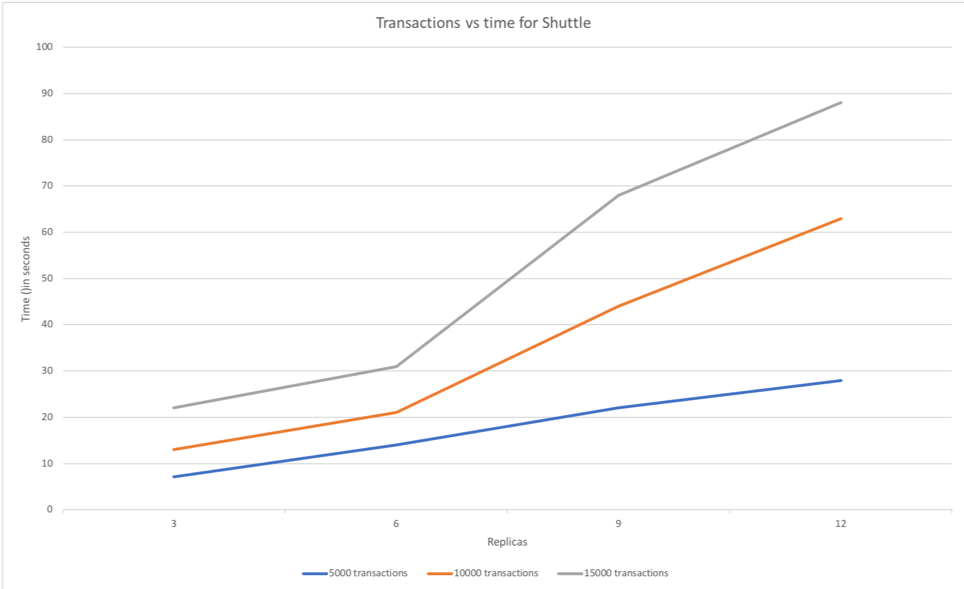
\includegraphics[width=0.3\textwidth]
    {ShuttleGraph}
\end{SCfigure}
\begin{SCfigure}
  \centering
  \caption{ Transaction volume vs time supporting f faults in Bchain3}
  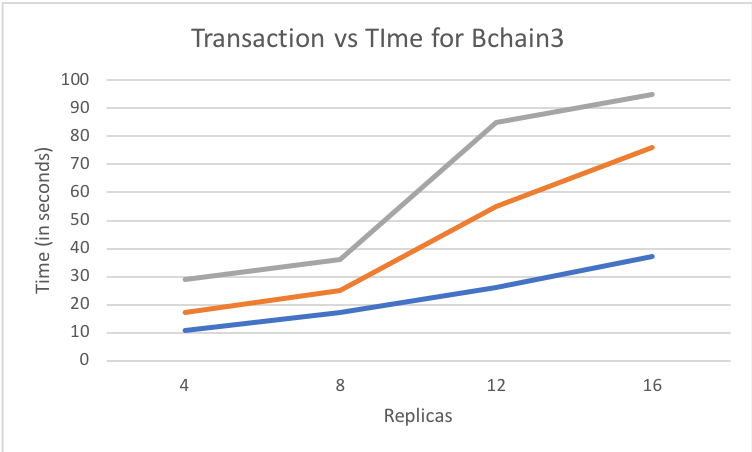
\includegraphics[width=0.3\textwidth]
    {BChain3}
\end{SCfigure}




%%%%%%%%%%%%%%%%%%%%%%%%%%%%%%%%%%%%%%%%%%%%%%%%%%%%%%%%%%%%%%%%%%%%%%%%%%%%%%%%

\section{Tweaking the original shuttle protocol}
We injected few tweaks in order to make the shuttle protocol more robust and evaluated our implementation with the original one. The client queries the head replica for each transaction. When the client issues a request, it starts a timer in order to maintain the liveness of the system. If the head replica does not respond to a client within the client's timer expires, the client resets the timer and queries each replica from the system. Each replica starts a timer and queries the head if the result that the client is requesting is not cached. The head replies to each replica with the result.
	
    We found this process to be inefficient because, each replica starts to query the head with the same query and the head replica starts servicing the same query multiple times. For this to make efficient, the head replica takes incoming queries in a FIFO queue, sends the computed query result to the replica that requested along the chain. Every replica that is expecting the re result will cache a copy and sends it back to the client. Since, each replica maintained a timer earlier, the process took some redundant and extra message exchanges. Following the protocol we developed reduced lot of redundant message exchanges and unnecessary timers.  


%%%%%%%%%%%%%%%%%%%%%%%%%%%%%%%%%%%%%%%%%%%%%%%%%%%%%%%%%%%%%%%%%%%%%%%%%%%%%%%%
\section{Conclusion}
To improve the integrity and availability of a service, the system should be replicated and Byzantine fault tolerant. However it comes under an increased cost. Just to support 1 fault, the data should be replicated on 4 servers and this number doubles to tolerate 2 faults. The protocol introduced in this paper reduces this number by t replicas. We also made the new protocol efficient by a small factor as discussed in the previous section.


%%%%%%%%%%%%%%%%%%%%%%%%%%%%%%%%%%%%%%%%%%%%%%%%%%%%%%%%%%%%%%%%%%%%%%%%%%%%%%%%
\begin{thebibliography}{99}

\bibitem{c1} Chain Replication for Supporting High Throughput and Availability. (Robert van Renesse and Fred B Schneider
\bibitem{c2} hBFT: Speculative Byzantine Fault Tolerance With Minimum Cost. Sisi Duan, Sean Peisert, and Karl Levitt. IEEE Transactions on Dependable and Secure
Computing (TDSC), March 2014.
\bibitem{c3} BChain: Byzantine Replication with High Throughput and Embedded Reconfiguration. Sisi Duan, Karl Levitt, Sean Peisert, and Haibin Zhang. Proceedings of the 18th International Conference on Principles of Distributed Systems (OPODIS), to appear, 2014
\bibitem{c4} Byzantine Fault Tolerance from Intrusion Detection. Sisi Duan, Karl Levitt, Hein Meling, Sean Peisert, and Haibin Zhang. To appear in Proceedings of the 33rd IEEE International Symposium on Reliable Distributed Systems (SRDS), pp. 253–264, 2014
\bibitem{c5} P2S: A Fault-Tolerant Publish/Subscribe Infrastructure. Tiancheng Change, Sisi Duan, Hein Meling, Sean Peisert, and Haibin Zhang. Proceedings of the 8th ACM International Conference on Distributed Event Based Systems (DEBS), pp. 189-197, 2014.
\bibitem(c6) Separating Agreement from Execution for Byzantine Fault Tolerant Services.

\end{thebibliography}




\end{document}
